% Hacer transparentes las partes ocultas (de otra forma se ocultan totalmente)
\setbeamercovered{transparent}

% Elegir el tema
%\usetheme{JuanLesPins}
%\useinnertheme{rounded}
\useinnertheme{circles}
\setbeamertemplate{blocks}[rounded]

% Poner los colores "lambda"
\DefineNamedColor{named}{ColorLambda}{named}{orange}
\usecolortheme[named={ColorLambda}]{structure}
\definecolor{grisnormal}{RGB}{170,170,170}
\definecolor{verdealerta}{RGB}{86,145,0}

% Otros colores
\setbeamercolor{top heading}{fg=black!30}
\setbeamercolor{section in head/foot}{fg=orange}
\setbeamercolor{subsection in head/foot}{fg=orange!50}
\setbeamercolor{item projected}{fg=black}
\setbeamercolor{description item}{fg=ColorLambda!50!black}
\setbeamercolor{alerted text}{fg=green!50!black}
\setbeamercolor{example text}{fg=ColorLambda!60!red!50!black}

 \setbeamercolor{block title}{use=structure,fg=white,bg=ColorLambda}
 \setbeamercolor{block title alerted}{use=alerted text,fg=white,bg=verdealerta}
 \setbeamercolor{block title example}{use=example text,fg=white,bg=grisnormal}
% 
 \setbeamercolor{block body}{parent=normal text,use=block title,bg=}
 \setbeamercolor{block body alerted}{parent=normal text,use=block title alerted,bg=}
 \setbeamercolor{block body example}{parent=normal text,use=block title example,bg=}


% Logo LambdaStream
\pgfdeclareimage[height=0.75cm]{LogoLambda}{LogoLambda}
%\pgfdeclareimage[height=1cm,width=12cm]{ovalo}{ovalo}
%\pgfdeclareimage[height=0.3cm]{separador}{separador}
% Encabezados y pies
\setbeamertemplate{headline}
{
%\vskip0.3cm
{\usebeamercolor[fg]{top heading} \hspace{0.5cm} \insertshortinstitute \hfill \insertshorttitle} \hspace{0.5cm}
\vspace{0.09cm}
{\usebeamercolor[fg]{top heading} \hrule}
\vspace{0.2cm}
\begin{tiny}{\usebeamercolor[fg]{section in head/foot} \hspace{0.5cm}{\textbf \insertsection}}\hfill %\begin{tiny}{\usebeamercolor[fg]{subsection in head/foot}\insertsubsectionnavigationhorizontal{0.2\paperwidth}{}{}}\end{tiny} 
{\usebeamercolor[fg]{subsection in head/foot}\insertsubsection} \hspace{0.5cm} \end{tiny}
\vskip-1cm
}

\setbeamertemplate{footline}{}


% 
% 
\setbeamertemplate{frametitle}
{
\leftskip=-20pt
%\vskip1cm
\vspace{1.2cm}
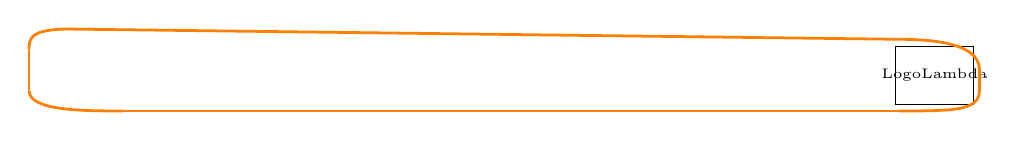
\begin{tikzpicture}
%\draw (0,0) node[anchor=west]{\pgfuseimage{ovalo}};
\draw[color=orange](0.4,0.1) node[anchor=west]{\textbf{\begin{footnotesize}\insertframetitle\end{footnotesize}}};
\draw[color=gray](0.6,-0.3) node[anchor=west]{\textbf{\begin{scriptsize}\insertframesubtitle\end{scriptsize}}};
\draw (11.5,-0.2) node{\pgfuseimage{LogoLambda}};
\begin{scope}[xscale=0.17, yscale=0.13, yshift=-5cm]
\draw[line width=1pt, color=orange] (3,8) .. controls (0,8) and (0,7) .. (0,6);
\draw[line width=1pt, color=orange] (0,6) .. controls (0,6) and (0,2) .. (0,2);
\draw[line width=1pt, color=orange] (0,2) .. controls (0,0) and (4,0) .. (7,0);
\draw[line width=1pt, 	color=orange] (7,0) .. controls (7,0) and (60,0) .. (65,0);
\draw[line width=1pt, color=orange] (65,0) .. controls (69,0) and (71,0) .. (71,2);
\draw[line width=1pt, color=orange] (71,2) .. controls (71,2) and (71,4) .. (71,4);
\draw[line width=1pt, color=orange] (71,4) .. controls (71,6) and (69,7) .. (65,7);
\draw[line width=1pt, color=orange] (65,7) .. controls (65,7) and (3,8) .. (3,8);
\end{scope}
\end{tikzpicture}

}
